\chapter{Energy and Optimization}
\label{sec:EnergyAndOptimization}
\index{optimization}

In this book, the description of locomotion models has been grounded in understanding the relevant dynamics through an energy description. Chapter \ref{sec:Introduction} introduced \textit{energy effectiveness} as a metric for locomotion. Chapter \ref{sec:PropertiesOfMotorsAndMuscles} describes the peak power that muscles can produce, and introduces the metric of \textit{metabolic cost}. The models developed in Chapter \ref{sec:ModelingLeggedLocomotion} include discussions of metabolic cost and energy loss from collisions. Energy is such an important aspect of locomtion is because, in general, locomotives move in such a way as to minimize the metabolic cost of locomotion. Likewise, the metabolic cost can be minimized for a \textit{model} of locomotion. If the metabolic cost of locomtion is available for a given dynamics model of locomotion, then it is possible to determine the parameters of the model that minimize that cost.

To arrive at a point where one can discover the parameters of a model that minimize the cost given by that model, some formal physics definitions are presented [chris: and muscle dynamics??].

\begin{verbatim}
[chris: ]people I should talk about
-bertram ruina 2000 paper on velocity relationsihps from constrained optimization
-
-
-
\end{verbatim}

\section{Energetics of Locomotion} %(notes page 39, 43-49)
\label{sec:EnergeticsOfLocomotion}
\index{energetics}

This section starts off with a review of some fundamental ideas in classical dynamics, but moves onto some thermodynamics concepts and a description of muscles that extends beyond what was presented in Chapter \ref{sec:PropertiesOfMotorsAndMuscles}.

In an introductory dynamics course, the equations of momentum conservation are developed with the understanding that only the external forces and torques appear in the equations for a given free body diagram. This fact may often be neglected, since the free body diagrams considered in such courses often do not have many internal forces. A locomotive, however, may move as a result of both internal forces and external forces. The free body diagram of a car only includes only external forces, such as gravity, normal forces, and friction (Figure \ref{fig:CarForces}). Of course, though, there are forces internal to the car as well. These forces do not appear in a free body diagram of the entire car, but would appear in a free body diagram of just the engine, or of just the transmission.

% FIGURE
\begin{figure}[h]		% h="here" t="top" b="bottom" p="separate page"
\begin{centering}
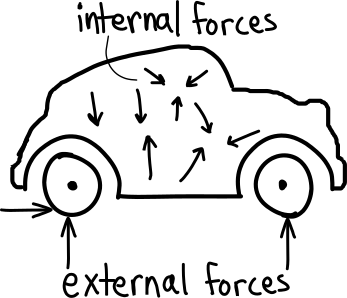
\includegraphics[width=0.3\textwidth]{Figures/CarForces}\par
\end{centering}
\caption{CarForces}
\label{fig:CarForces}
\end{figure}
%

Humans and animals are like locomotives in that they are not propelled solely by external forces, as is the case with point masses. What implications does this have for energy, and more intuitively, power? It is enlightening to develop equations for power with the distinction between internal and external forces. The instantaneous power required to force a particle that is traveling at a velocity $\vv$ is

\begin{align}
P &= \vF_{tot} \cdot \vv \\
 &= m\va \cdot \vv = \frac{d}{dt} \left(\frac{m v^2}{2}\right) = \KEdot
\end{align}

where the chain rule of differentiation has been employed ($dv^2/dt = 2v(dv/dt)$). This provides the logical result for a particle, that $P = \KE$. f course the total force in this case is also the total external force, since a particle cannot have any internal forces. Likewise, the power required to move a collection of particles (or a system of particles and rigid bodies) can be written as

\begin{align}
P_{tot} &= \sum_i \vF_i \cdot \vv_i \\
&= \sum_i \frac{d}{dt}\left(\frac{m_i v_i^2}{2}\right) = \sum_i \KEdot_i 
\label{eq:PowerCollectionOfParticles}
\end{align}

where $\vF$ is the total force on particle $i$. Equation \ref{eq:PowerCollectionOfParticles} can be used to describe the power developed with a system as simple as a two-particle system, or as complicated as a car (in the latter case, the system is comprised mostly of rigid bodies, in which case the forces and velocities are of the centers of mass of the rigid bodies). With internal and external forces are written separately, the power can be related to the time rate of change of kinetic energy as follows

\begin{align}
P_{tot} &= \sum_i (\vF_{i}^{int} + \vF_{i}^{ext}) \cdot \vv_{i} \\
&= \KEdot = \KEdot_{/G} + \KEdot_{G}
\label{eq:PowerInternalExternal}
\end{align}

where $\vF_i^{int}$ and $\vF_i^{ext}$ are respectively the total internal and external forces acting on particle $i$, $\KEdot$ is the time rate of change of the total kinetic energy of the system, $\KEdot_{/G}$ is the sum of the kinetic energy of each particles (or rigid bodies) with respect to the center of mass of the system, and $\KEdot_{G}$ is the kinetic energy of the center of mass of the system

Accordingly, these last two terms are given by 
\begin{align}
\KEdot_{/G} &= \frac{d}{dt} \sum_{i} \frac{m_i}{2}(v_{i} - v_{G})^{2} \\
\KEdot_{G} &= m_{T} \frac{d}{dt} v_{G}^{2}
\end{align}

where $v_{G}$ is the speed of the center of mass of the system, and $m_{T}$ is the total mass of the system ($\sum m_i$).

Equation \ref{eq:PowerInternalExternal} describes power as a sum of internal forces and external forces, and describes the time rate of change of kinetic energy as a sum of a ``relative'' kinetic energy, and an ``absolute'' kinetic energy. It may seem that these terms correspond to each other; that the internal forces cause an internal power equivalent to $\KEdot_{G}$ and that the external forces cause an external power equivalent to $\KEdot_{/G}$. If a car is in neutral and the driver depresses the accelerator, then the car has internal forces that contribute to an internal power that \textit{is} equivalent to $\KEdot_{/G}$, there is no external power and $\KEdot_{G} = m_{T}(0)^2/2 = 0$, and the proposed correspondence holds. However, this logic is incorrect in general. Once again, consider the car in Figure \ref{fig:CarForces}. A free body diagram of this car illustrates that if the car is accelerating, its acceleration is a result of the horizontal external force acting at the bottom of its wheels. Additionally, $\KEdot_{G}$ is increasing since it is a function of $v_{G}$. It may seem that this is the external force that contributes to $\KEdot_{G}$. However, the velocity of a wheel at the point at which the horizontal external force is instantaneously zero (no-slip condition). Thus, this external force does not produce any power. Instead, $\KEdot_{G}$ arises from internal forces.

This delicacy of this distinction is also revealed by the system described in Figure \ref{fig:ParticleExplosion}. A particle explodes on a surface, and separates into two equal-mass particles. One particle flies off to the right at velocity $\vv_m$. The other particle is anchored to the surface, and the surface and particle subsequently travel to the right at $\vv_m$. In this case, the center of mass of the two-particle system does not move, so $\KEdot_{G} = 0$. There is an external force from the surface on the right particle, $F_{ext}$, that is also an external force on the . [chris: actually this example doesnt make sense. if the wall is moving, it also has a mass and so...i guess im confused by what anchoring actually means].

[chris: it is possible to write Fext,tot*vg = Ekg?]


% FIGURE
\begin{figure}[h]		% h="here" t="top" b="bottom" p="separate page"
\begin{centering}
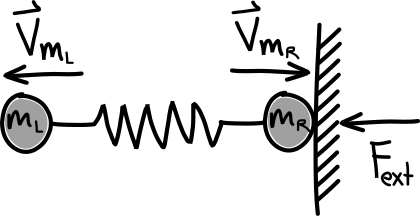
\includegraphics[width=0.4\textwidth]{Figures/ParticleExplosion}\par
\end{centering}
\caption{ParticleExplosion}
\label{fig:ParticleExplosion}
\end{figure}
%

A locomotive can be approximated as a system of linked rigid bodies. The time rate of change of the total kinetic energy of a locomotive $\KEdot$ can be expressed in terms of the forces and moments acting on the rigid bodies that compose a locomotive in a way that is slightly more detailed than Equation \ref{eq:PowerInternalExternal}. Logically, a locomotive is modeled better as a system of linked rigid bodies than as a collection of point-masses (especially if the aim is to understand how muslces affect the motion of the locomotive). Again, the locomotive has both internal and external forces (and internal and external forces). Starting from Equation \ref{eq:PowerInternalExternal} and noting that $\vv_i = \vv_{G} + \vv_{i/G}$ and $\vv_{i/G} = \vomega_{G} \times \vec{\mathbf{r}}_{i/G}$, $\KEdot$ can be written as 

\begin{equation}
\KEdot = \sum_{i} (\vF_{i}^{int} + \vF_{i}^{ext} ) \cdot ( \vv_{G} + \vomega_{G} \times \vec{\mathbf{r}}_{i/G})
\end{equation}

The right hand side can be expanded, and one of the resulting terms is $\sum \vF_{i}^{int} \cdot (\vomega_{G} \times \vec{\mathbf{r}}_{i/G})$. Using vector properties, this term can be rewritten as $\vomega \cdot \sum \vec{\mathbf{r}}_{i/G} \times \vF_{i}^{int}$. This term vanishes, since according to Newton's second law, each internal force on a given link also has an equal and opposite force acting on some other link. Through other simplifications, $\KEdot$ can eventually be written as

\begin{equation}
\KEdot = \sum_{i} \vF_{i}^{ext} \cdot \vv_{i} + \sum_{i} \vomega_{G} \times \vM_{i}^{ext}
\end{equation}

Thus, the energy of the locomotive only depends on external forces and moments. This conclusion seems to contradict the earlier statement that indicates that the kinetic energy of the center of mass of the locomotive can recieve contribution from internal forces and internal power. [chris: doesn't it?] Consult any standard advanced dynamics textbook for a more thorough understanding of this derivation.

In the context of internal forces an internal power, it makes sense to describe a model of a locomotive using the First Law of Thermodynamics. The total energy of a locomotive, a closed system, is the sum of its kinetic energy $\KE$ and its internal energy $U$ (potential energy is neglected). The time rate of change of the total energy of a locomotive is given as

\begin{equation}
\KEdot + \dot{U} = P^{ext} + \dot{Q} + \dot{W}
\end{equation}


The external power $P^{ext}$ arises from friction, the heat input term $\dot{Q}$ arises from temperature differences, and the work term $\dot{W}$ arises from external work input to the system. Friction and the work term can be neglected, since sliding does not often occur with locomotives (thus no power is lost to friction), and no odd external work inputs are considered. The time rate of change of the internal energy of the locomotive can be expressed as

\begin{equation}
\dot{U} = -P^{int} + [\mbox{heat prod}] + \dot{E}_{chem}
\end{equation}

Combining Equations

\begin{equation}
P^{int} + (\dot{Q} - [\mbox{heat prod}]) - \dot{E}_{chem} = \KEdot_{/G} + \KEdot_{G}
\end{equation}

Typically, $\dot{Q} < 0$ and $\dot{E}_{chem} < 0$. [chris: i can't really do this section now, esp cuz idk how the thermodynamics is used later on. What is Echem?. i understand that people release heat so that's why q islesthan 0. i don't know why pint is less than zero.]

The general ideas presented so far can now be applied in a more direct fashion to humans and animals. Just as the engine in an automotive gives rise to internal forces and power that ultimately move the automobile, the muscles in an animal give rise to internal power that move the locomotive. The following assumptions and simplifications are made

\begin{itemize}
\item \textbf{Negligible gravity power:} Logically, this text is only concerned with mostly horizontal translation of the locomotion's center of mass. Thus, the force of gravity does not create a substantial external power (the force of gravity is perpendicular to the center of mass's velocity, and so the dot product of the two quantities is small). This would not be true for locomotion down or up a substantial incline.
\item \textbf{Negligible friction power:} Energy is not removed from the system (the locomotive) by either air friction or sliding. Sliding can occur, but only for a frictionless contact.
\item \textbf{Negligible ground deformation:} Energy is not removed from the system as a result of the collisions of limbs with the ground.
\end{itemize}

To a large extent, these assumptions are made so that the $P^{ext}$ term in the thermodynamic energy balance can be neglected. Additionally, internal friction is also neglected. This friction can come from frictional joints or from the inelastic compression of non-muscle soft tissue. As a result, the only relevant power source (or sink) in the system is that generated by muslces or by joints in the locomotive. That is,

\begin{equation}
P = P^{int} = \sum_{i} P_{i}^{joint} + \sum_{j} P_{j}^{musc}
\end{equation}

A joint, such as an elbow, can be analyzed by first developing a free body diagram of the joint, as in Figure \ref{fig:ElbowFBD}.

%
% FIGURE
\begin{figure}[h]		% h="here" t="top" b="bottom" p="separate page"
\begin{centering}
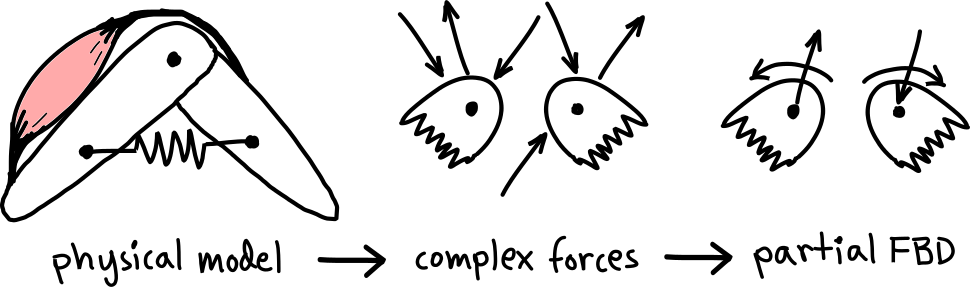
\includegraphics[width=0.8\textwidth]{Figures/ElbowFBD}\par
\end{centering}
\caption{ElbowFBD}
\label{fig:ElbowFBD}
\end{figure}
%

The muscle can be modeled as a spring that acts between two points on different bones. There are likely many forces acting on a joint, but they can be reduced to an equivalent single force and moment. The power generated at the joint is then given by the resultant moment and the angular velocity at which the joint is opening or closing.

\begin{equation}
P_{joint} = \vM \cdot \vomega_{rel}
\end{equation}

% FIGURE
\begin{figure}[h]		% h="here" t="top" b="bottom" p="separate page"
\begin{centering}
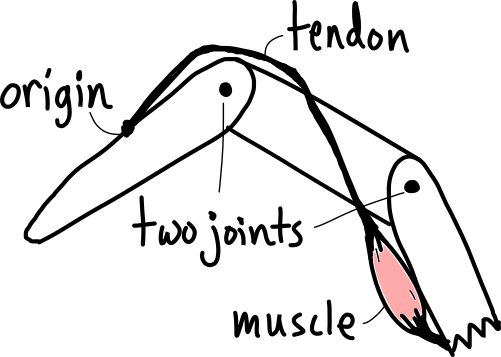
\includegraphics[width=0.3\textwidth]{Figures/TwoJoints}\par
\end{centering}
\caption{TwoJoints}
\label{fig:TwoJoints}
\end{figure}
%

Some muscles act through two joints, as shown in Figure \ref{fig:TwoJoints}. In this case, the muscle is connected to the farther bone through a tendon. The power generated by the muscle is approximated by

\begin{equation}
P^{musc} = -T \dot{l}
\end{equation}

where $T$ is the tension in the muscle and $l$ is the length of the muscle, as in Figure \ref{fig:OneMuscle}.

% FIGURE
\begin{figure}[h]		% h="here" t="top" b="bottom" p="separate page"
\begin{centering}
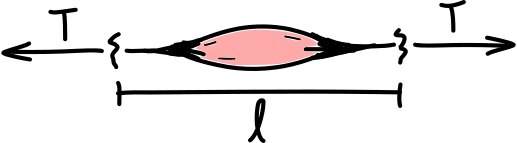
\includegraphics[width=0.4\textwidth]{Figures/OneMuscle}\par
\end{centering}
\caption{OneMuscle}
\label{fig:OneMuscle}
\end{figure}
%

By analyzing muscles in this way, it is possible to quantify the overal level of muscle activity occuring in a locomotive. However, this process would be arduous. It makes much more sense to deductively determine the muscle activity by finding $P^{int}$. This can be measured externally through experiments. The simplest type of experiment is having a locomotive perform a gait on a force plate, as shown in Figure \ref{fig:ForcePlate}. A likely setup is to place the force plate under a tread mill on which the locomotive moves in place. The force plate then records the vertical force exerted by the locomotive $\vF^{tot}(t)$ as a function of time.

% FIGURE
\begin{figure}[h]		% h="here" t="top" b="bottom" p="separate page"
\begin{centering}
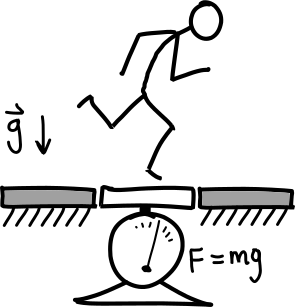
\includegraphics[width=0.25\textwidth]{Figures/ForcePlate}\par
\end{centering}
\caption{ForcePlate}
\label{fig:ForcePlate}
\end{figure}
%

The recorded force can be divided into two parts.

\begin{equation}
\vF^{tot}(t) = \vF^{G} + mg \uj
\end{equation}

where $\vF^{G}$ is the reaction force of the ground on the locomotive. The acceleration of the center of mass $\va_{G}(t)$ is given by $\vF^{tot}/m_{tot}$. The velocity, which is required to find power, is determined by integrating this acceleration over time.

\begin{equation}
\vv(t) = \vv(t=0) + \int_{0}^{t} \va(\tau) d\tau
\label{eq:VelocityIntegral}
\end{equation}

Note that the force plate measures a vertical force only. As a result, the acceleration provided is a vertical acceleration. If the locomotive maintains a constant horizontal velocity, then the error from using the force plate measurement to calculate $\va(t)$ is minimal. To find the velocity at any time, the initial velocity must be known. If the motion is assumed to be periodic, then the integral of the velocity over a period of the gait is equal to the locomotive's average velocity. Additionally, the integral of the acceleration over a period of the gait is zero.

\begin{align}
\bar{\vv} &= \frac{1}{T}\int_{0}^{T} \vv(\tau)d\tau \notag \\
&= \frac{1}{T} \int_0^{T} \left( \vv(0) + \int_0^t \va(t') dt' \right) dt \\
0 &= \int_{0}^{T} \va(t)dt
\label{eq:VelocityIntegralAverage}
\end{align}

Equation\ref{eq:VelocityIntegralAverage} can be solved for the initial velocity, assuming that the average velocity can also be measured. The quantities $\vv_{G}$ and $\va_{G}$ can be used to calculate $\KEdot_{G}$

\begin{equation}
\KEdot_{G}(t) = m_{tot} \vv_{G} \cdot \va_{G}
\end{equation}

In biomechanics, an ``external power'' is often calculated as

\begin{align}
\mbox{''external power''} &= m_{tot} \vv_{G} \cdot \va_{G} - m_{tot} g \uj \cdot \vv_{G} \notag \\
&= \KEdot_{G} - m_{tot} g \uj \cdot \vv_{G}
\end{align}

Remember that under the assumptions made earlier, $P^{ext}(t)$ is actually approximately zero. This still holds. [chris: I thought we were after internal power, not external power]

A better experiment can be performed if two force plates are used. Kuo and Donnelin
Keonig's Theorem

\begin{align}
P_{1} &= \vF_{1} \cdot \vv_{G} \\
P_{2} &= \vF_{2} \cdot \vv_{G}
\end{align}

[chris: check m_{tot} syntax]

\section{Energy Optimization} %(notes page 49-54)
\label{sec:EnergyOptimization}
\index{optimization}

John Bertram

% FIGURE
\begin{figure}[h]		% h="here" t="top" b="bottom" p="separate page"
\begin{centering}
\includegraphics[width=0.4\textwidth]{Figures/Optimization}\par
\end{centering}
\caption{Optimization}
\label{fig:Optimization}
\end{figure}
%

% FIGURE
\begin{figure}[h]		% h="here" t="top" b="bottom" p="separate page"
\begin{centering}
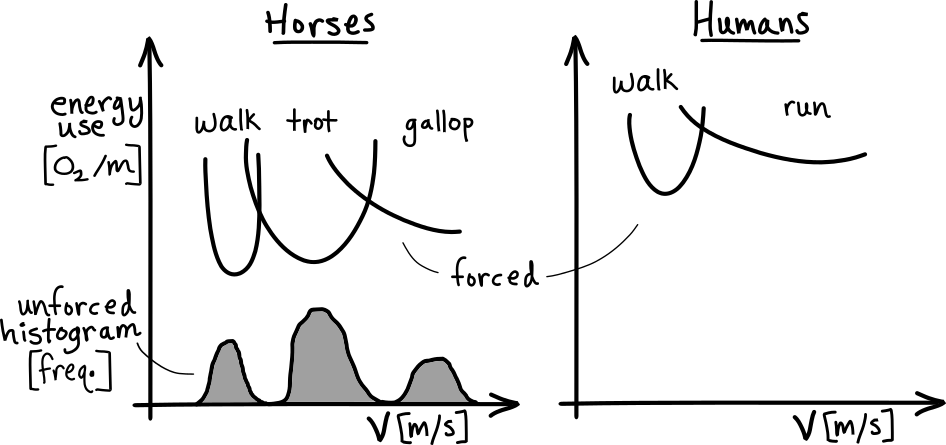
\includegraphics[width=0.8\textwidth]{Figures/HorseLocomotion}\par
\end{centering}
\caption{HorseLocomotion}
\label{fig:HorseLocomotion}
\end{figure}
%


% FIGURE
\begin{figure}[h]		% h="here" t="top" b="bottom" p="separate page"
\begin{centering}
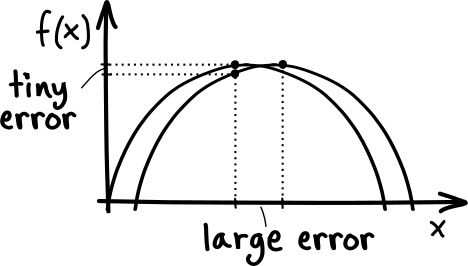
\includegraphics[width=0.4\textwidth]{Figures/BadPredictor}\par
\end{centering}
\caption{BadPredictor}
\label{fig:BadPredictor}
\end{figure}
%

% FIGURE
\begin{figure}[h]		% h="here" t="top" b="bottom" p="separate page"
\begin{centering}
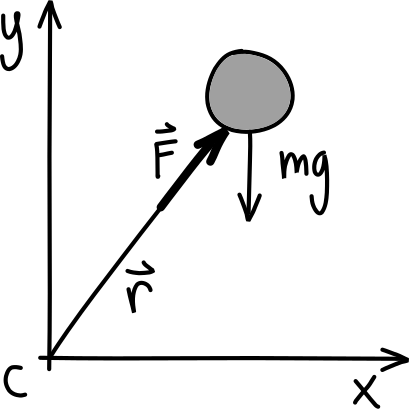
\includegraphics[width=0.25\textwidth]{Figures/PointMass}\par
\end{centering}
\caption{PointMass}
\label{fig:PointMass}
\end{figure}
%


% FIGURE
\begin{figure}[h]		% h="here" t="top" b="bottom" p="separate page"
\begin{centering}
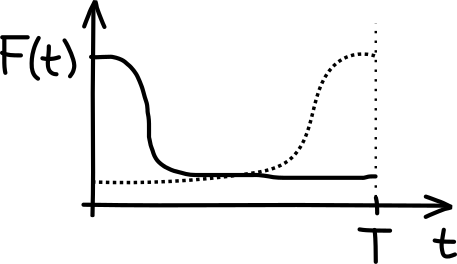
\includegraphics[width=0.4\textwidth]{Figures/ForceOptimization}\par
\end{centering}
\caption{ForceOptimization}
\label{fig:ForceOptimization}
\end{figure}
%

\section{Optimal Control} %(notes page 54-60, 64)
\label{sec:OptimalControl}
\index{control!optimal}

% FIGURE
\begin{figure}[h]		% h="here" t="top" b="bottom" p="separate page"
\begin{centering}
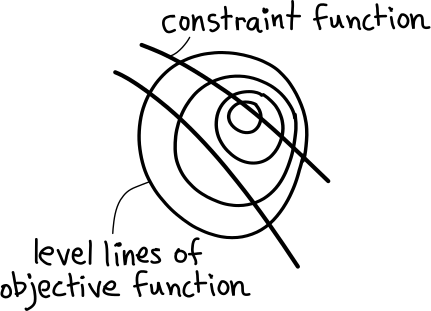
\includegraphics[width=0.4\textwidth]{Figures/ObjectiveFunction}\par
\end{centering}
\caption{ObjectiveFunction}
\label{fig:ObjectiveFunction}
\end{figure}
%


% FIGURE
\begin{figure}[h]		% h="here" t="top" b="bottom" p="separate page"
\begin{centering}
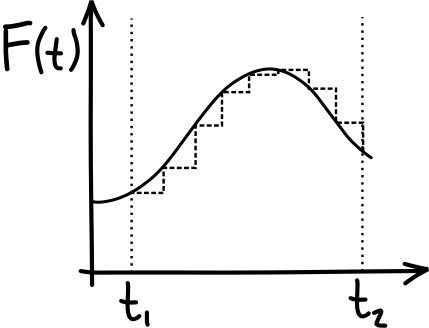
\includegraphics[width=0.35\textwidth]{Figures/PiecewiseConstant}\par
\end{centering}
\caption{PiecewiseConstant}
\label{fig:PiecewiseConstant}
\end{figure}
%


% FIGURE
\begin{figure}[h]		% h="here" t="top" b="bottom" p="separate page"
\begin{centering}
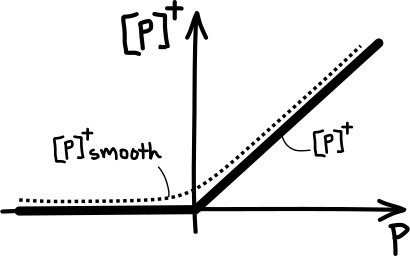
\includegraphics[width=0.4\textwidth]{Figures/SmoothedFunction}\par
\end{centering}
\caption{SmoothedFunction}
\label{fig:SmoothedFunction}
\end{figure}
%

% FIGURE
\begin{figure}[h]		% h="here" t="top" b="bottom" p="separate page"
\begin{centering}
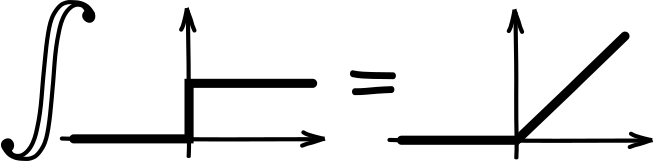
\includegraphics[width=0.4\textwidth]{Figures/IntegralFunction}\par
\end{centering}
\caption{IntegralFunction}
\label{fig:IntegralFunction}
\end{figure}
%

% FIGURE
\begin{figure}[h]		% h="here" t="top" b="bottom" p="separate page"
\begin{centering}
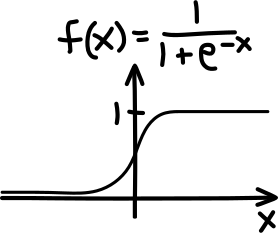
\includegraphics[width=0.25\textwidth]{Figures/LogisticFunction}\par
\end{centering}
\caption{LogisticFunction}
\label{fig:LogisticFunction}
\end{figure}
%

READ RUINA'S RANT ONLINE

SNOPT and the like. $\int{x}$
\index{SNOPT}
